% DPCN Assignment 2 report (Group 12). Compile with XeLaTeX (Overleaf: Menu -> Compiler -> XeLaTeX) or Tectonic.
% All numbers come from numbers.tex, and the figures and tables from figures/ and tables/; all are written by
% scripts/build_report.py from the analysis outputs, so re-run that script after changing any analysis.
\documentclass[10pt,twocolumn,a4paper]{article}

% --- Essential Packages ---
\usepackage{fontspec}
\setmainfont{texgyretermes}[Extension=.otf, UprightFont=*-regular, BoldFont=*-bold, ItalicFont=*-italic, BoldItalicFont=*-bolditalic]
\usepackage{unicode-math}
\setmathfont{texgyretermes-math.otf}
\usepackage[margin=0.62in, top=0.6in, bottom=0.7in, columnsep=16pt]{geometry}
\usepackage{booktabs}
\usepackage{graphicx}
\usepackage{caption}
\usepackage{hyperref}
\usepackage{microtype}
\usepackage{tikz}
\usetikzlibrary{arrows.meta, positioning}
\usepackage{xcolor}
\usepackage{enumitem}
\usepackage{titlesec}
\usepackage{array}

% --- Hyperref Setup ---
\hypersetup{colorlinks=true, linkcolor=blue!70!black, citecolor=blue!70!black, urlcolor=blue!70!black}

% --- Custom Formatting & Spacing ---
\setlength{\parindent}{1em}
\setlength{\parskip}{0.1em}
\titlespacing*{\section}{0pt}{1.0ex plus 0.3ex minus 0.1ex}{0.4ex plus 0.1ex}
\titlespacing*{\subsection}{0pt}{0.8ex plus 0.2ex minus 0.1ex}{0.3ex plus 0.1ex}
\titleformat*{\section}{\large\bfseries}
\titleformat*{\subsection}{\normalsize\bfseries}
\captionsetup{font=small, labelfont=bf, skip=3pt}
\setlength{\textfloatsep}{8pt plus 2pt minus 2pt}
\setlength{\floatsep}{6pt plus 2pt minus 2pt}
\setlength{\dbltextfloatsep}{8pt plus 2pt minus 2pt}
\setlength{\abovedisplayskip}{3pt}\setlength{\belowdisplayskip}{3pt}
\setlength{\abovedisplayshortskip}{2pt}\setlength{\belowdisplayshortskip}{2pt}
\renewcommand{\arraystretch}{1.05}
\setlist{noitemsep, topsep=1pt, leftmargin=1.1em}
\renewcommand{\topfraction}{0.9}\renewcommand{\dbltopfraction}{0.9}\renewcommand{\textfraction}{0.06}
\renewcommand{\floatpagefraction}{0.7}\renewcommand{\dblfloatpagefraction}{0.7}\renewcommand{\bottomfraction}{0.6}
\setcounter{totalnumber}{6}\setcounter{topnumber}{4}\setcounter{bottomnumber}{3}
\makeatletter
\setlength{\@fptop}{0pt}\setlength{\@fpsep}{8pt}\setlength{\@dblfptop}{0pt}\setlength{\@dblfpsep}{10pt}
\makeatother
\raggedbottom
% Generated by scripts/build_report.py from the analysis outputs. Do not edit by hand; re-run the script.
\newcommand{\nFaculty}{743}
\newcommand{\nFacT}{415}
\newcommand{\nFacS}{328}
\newcommand{\nPapers}{18{,}343}
\newcommand{\nPapT}{9{,}184}
\newcommand{\nPapS}{9{,}206}
\newcommand{\nJoint}{47}
\newcommand{\nLinks}{961}
\newcommand{\nInternal}{23{,}822}
\newcommand{\yrA}{1{,}071}
\newcommand{\yrB}{1{,}924}
\newcommand{\growth}{1.8}
\newcommand{\qIfFiveT}{21.7\%}
\newcommand{\qIfFiveS}{23.6\%}
\newcommand{\pQIfFive}{0.008}
\newcommand{\nQIfFiveT}{1{,}586}
\newcommand{\nQIfFiveS}{1{,}481}
\newcommand{\qIfTenT}{4.6\%}
\newcommand{\qIfTenS}{4.3\%}
\newcommand{\pQIfTen}{0.47}
\newcommand{\nQIfTenT}{337}
\newcommand{\nQIfTenS}{272}
\newcommand{\ifTenQOne}{609 of 632}
\newcommand{\ifFiveNotQOne}{32\%}
\newcommand{\lessTenT}{99.1\%}
\newcommand{\lessTenS}{99.4\%}
\newcommand{\nLessTenT}{9{,}100}
\newcommand{\nLessTenS}{9{,}149}
\newcommand{\bigCite}{2\%}
\newcommand{\mathQOneLow}{90\%}
\newcommand{\fwciEffect}{+1.2}
\newcommand{\pRobust}{0.22}
\newcommand{\pClust}{0.63}
\newcommand{\asstT}{48\%}
\newcommand{\asstS}{31\%}
\newcommand{\gapRaw}{+33\%}
\newcommand{\gapRank}{+24\%}
\newcommand{\pProf}{0.71}
\newcommand{\brS}{CSE and EEE}
\newcommand{\brT}{Chemical and Mathematics}
\newcommand{\qOneT}{35.2\%}
\newcommand{\qOneS}{38.3\%}
\newcommand{\ifFiveT}{33.0\%}
\newcommand{\ifFiveS}{33.8\%}
\newcommand{\citT}{15.2}
\newcommand{\citS}{13.6}
\newcommand{\hT}{7}
\newcommand{\hS}{9}
\newcommand{\pH}{0.010}
\newcommand{\papMedT}{19}
\newcommand{\papMedS}{31}
\newcommand{\pFwciPers}{0.16}
\newcommand{\aiA}{9.1}
\newcommand{\aiB}{20.3}
\newcommand{\aiOA}{4.7}
\newcommand{\aiOB}{12.7}
\newcommand{\aiDeptA}{10}
\newcommand{\aiDeptB}{15}
\newcommand{\aiDeptN}{18}
\newcommand{\nBranch}{10}
\newcommand{\topTrichy}{7}
\newcommand{\topReview}{4}
\newcommand{\zeroIndeg}{58\%}
\newcommand{\maxIndeg}{40}
\newcommand{\alphaIn}{2.9}
\newcommand{\selfShare}{86\%}
\newcommand{\flowRT}{36{,}970}
\newcommand{\flowGT}{43{,}057}
\newcommand{\ratioT}{0.86}
\newcommand{\flowRS}{30{,}349}
\newcommand{\flowGS}{37{,}191}
\newcommand{\ratioS}{0.82}
\newcommand{\cIIT}{0.40}
\newcommand{\cCSIR}{0.33}
\newcommand{\cUni}{1.32}
\newcommand{\citeTS}{315}
\newcommand{\citeST}{319}
\newcommand{\partT}{465}
\newcommand{\partS}{472}
\newcommand{\indCollT}{35\%}
\newcommand{\indCollS}{31\%}
\newcommand{\forCollT}{17\%}
\newcommand{\forCollS}{14\%}
\newcommand{\uniShare}{56\%}
\newcommand{\geoJoint}{37}
\newcommand{\geoCite}{16}
\newcommand{\geoElJ}{38}
\newcommand{\geoElC}{11}
\newcommand{\nConn}{540}
\newcommand{\nNodes}{657}
\newcommand{\nLCC}{491}
\newcommand{\nCross}{28}
\newcommand{\crossPct}{2.9\%}
\newcommand{\maxDeg}{22}
\newcommand{\bridgeT}{54\%}
\newcommand{\bridgeS}{44\%}
\newcommand{\randT}{8\%}
\newcommand{\randS}{10\%}
\newcommand{\nComm}{45}
\newcommand{\modQ}{0.85}
\newcommand{\commTen}{19}
\newcommand{\nmi}{0.68}
\newcommand{\nmiRand}{0.24}
\newcommand{\assortBranch}{0.66}
\newcommand{\assortRank}{0.07}
\newcommand{\zRank}{4.3}
\newcommand{\apl}{6.1}
\newcommand{\aplR}{4.5}
\newcommand{\clust}{0.21}
\newcommand{\clustR}{0.011}
\newcommand{\clustRatio}{20}
\newcommand{\swSigma}{14.8}
\newcommand{\assortDeg}{0.20}
\newcommand{\rcRho}{3.7}
\newcommand{\trans}{0.21}
\newcommand{\aExp}{1.65}
\newcommand{\aRsq}{0.998}
\newcommand{\degA}{1.67}
\newcommand{\degB}{3.48}
\newcommand{\yrDegMin}{1.7}
\newcommand{\yrDegMax}{2.0}
\newcommand{\diamPeak}{19}
\newcommand{\diamYear}{2018}
\newcommand{\diamNow}{9}
\newcommand{\aplPeak}{11.2}
\newcommand{\aSixMin}{1.19}
\newcommand{\aSixMax}{1.74}
\newcommand{\aTrOwn}{1.61}
\newcommand{\aSuOwn}{1.70}
\newcommand{\lpAUC}{0.90, 0.87, 0.90}
\newcommand{\lpTop}{19, 14, 9}
\newcommand{\lpLiftMin}{15}
\newcommand{\lpLiftMax}{22}
\newcommand{\lpMatches}{42}
\newcommand{\lpOut}{27}
\newcommand{\lpBase}{0.05}
\newcommand{\rhoSix}{−1.00}
\newcommand{\pSix}{0.003}
\newcommand{\selfMin}{85}
\newcommand{\selfMax}{92}
\newcommand{\lamOneT}{6.055}
\newcommand{\lamOneS}{7.876}
\newcommand{\lamNBT}{4.732}
\newcommand{\lamNBS}{6.424}
\newcommand{\bcT}{0.211}
\newcommand{\bcS}{0.156}
\newcommand{\reachT}{1.9 / 3.9 / 10.1}
\newcommand{\reachS}{2.8 / 8.4 / 24.8}
\newcommand{\KcT}{0.264}
\newcommand{\KcS}{0.203}
\newcommand{\eigR}{670}
\newcommand{\eigRw}{130}
\newcommand{\stuN}{2{,}917}
\newcommand{\stuAll}{21{,}260}
\newcommand{\stuPct}{16\%}
\newcommand{\stuMedT}{0.63}
\newcommand{\facMedT}{0.63}
\newcommand{\stuMedS}{0.48}
\newcommand{\facMedS}{0.65}
\newcommand{\privPer}{43}
\newcommand{\pubPer}{37}
\newcommand{\privP}{0.28}
\newcommand{\privNear}{31}
\newcommand{\pubNear}{21}
\newcommand{\forEff}{+18}
\newcommand{\forUni}{+17}
\newcommand{\iitEff}{+3}
\newcommand{\teamA}{0.72}
\newcommand{\teamB}{2.09}
\newcommand{\teamBig}{1}
\newcommand{\manipShare}{5.0\%}
\newcommand{\manipRho}{0.999}
\newcommand{\manipN}{117{,}909}
\newcommand{\nFindings}{28}
\newcommand{\nPicked}{11}
\newcommand{\flowLateMin}{1.03}
\newcommand{\flowLateMax}{1.35}
\newcommand{\assortNull}{$-$0.02}
\newcommand{\assortZ}{6.9}
\newcommand{\kerA}{0.35}
\newcommand{\kerT}{0.26}
\newcommand{\kerS}{0.32}
\newcommand{\kerOne}{0.26}
\newcommand{\kerNine}{0.47}
\newcommand{\richA}{0.75}
\newcommand{\bmfT}{0.251}
\newcommand{\bmfS}{0.196}
\newcommand{\bLamT}{0.165}
\newcommand{\bLamS}{0.127}
\newcommand{\kOneT}{3.15}
\newcommand{\kTwoT}{15.71}
\newcommand{\kOneS}{3.83}
\newcommand{\kTwoS}{23.39}
\newcommand{\gravJ}{0.70}
\newcommand{\gravC}{0.17}
\newcommand{\superPct}{11}
\newcommand{\superCut}{9}
\newcommand{\superShare}{52}
\newcommand{\superDept}{89}
\newcommand{\otherDept}{66}
\newcommand{\onePaper}{40}
\newcommand{\renewThree}{57}
\newcommand{\stillActive}{27}
\newcommand{\renewOne}{51}
\newcommand{\renewFive}{81}
\newcommand{\nNew}{257}
\newcommand{\newIso}{46}
\newcommand{\newIsoT}{52}
\newcommand{\newIsoS}{30}
\newcommand{\newDept}{76}
\newcommand{\nTri}{314}
\newcommand{\triFilled}{58}
\newcommand{\triTeam}{36}
\newcommand{\triPapers}{8.8}
\newcommand{\nGroups}{112}
\newcommand{\groupsFive}{22}
\newcommand{\groupsAll}{4}
\newcommand{\groupsOne}{36}
\newcommand{\brokerOther}{43}
\newcommand{\allOther}{14}
\newcommand{\brokerTop}{14}
\newcommand{\nRanked}{439}
\newcommand{\rankMin}{10}
\newcommand{\rankRho}{0.993}
\newcommand{\giniC}{0.64}
\newcommand{\giniP}{0.49}
\newcommand{\topTenC}{45\%}
\newcommand{\botHalfC}{7\%}
\newcommand{\nFormer}{99}
\newcommand{\movedIIT}{8}
\newcommand{\movedNIT}{7}
\newcommand{\asstFirst}{12\%}
\newcommand{\asstLast}{50\%}
\newcommand{\profLast}{58\%}
\newcommand{\confEff}{−35}
\newcommand{\qThreeEff}{−44}
\newcommand{\qTwoEff}{−27}
\newcommand{\oaShare}{22\%}
\newcommand{\oaGold}{+13}
\newcommand{\oaGreen}{+10}
\newcommand{\oaDiamond}{−12}
\newcommand{\homeShare}{13.2\%}
\newcommand{\homeEff}{+1.5}
\newcommand{\nDoubt}{463}
\newcommand{\doubtPap}{−1.6}
\newcommand{\doubtCit}{−0.7}
\newcommand{\priceAll}{38}
\newcommand{\priceRho}{0.17}
\newcommand{\priceA}{32}
\newcommand{\priceB}{40}
\newcommand{\priceYA}{2016}
\newcommand{\priceYB}{2025}
\newcommand{\internalSelf}{86}


% --- Document Title & Metadata ---
\title{\vspace{-1.6em}\textbf{\Large Dynamics and Processes on Complex Networks (DPCN)}\\\vspace{0.2em}
\textbf{\large Assignment 2: Research Mapping of NIT Trichy and NIT Surathkal, 2016--2026}\\\vspace{0.2em}
\normalsize Publication Statistics, Citation and Co-authorship Networks, and Phase II Analyses}
\author{\textbf{Group 12 (Top NITs cluster)}\\[0.2em]\normalsize
\begin{tabular}{ccc}
\textbf{Ampilli Sai Venkata Naga Bhargav} & \textbf{Chaitanya Thogata} & \textbf{Pasumarthy Deepak}\\
(\textit{2023112014}) & (\textit{2023113018}) & (\textit{2023101109})
\end{tabular}}
\date{\vspace{-1.8em}}

\begin{document}
\maketitle

% ==============================================================================
\section{Team, Code and Dashboard}
\label{sec:team}
Group 12 studied the science and engineering faculty of \textbf{NIT Tiruchirappalli (Trichy)} and \textbf{NIT Karnataka (Surathkal)} for 2016--2026.
Code, data and all outputs are at \url{https://github.com/saiXbhargav/DPCN_assignment2}, and the interactive dashboard (16 tabs, both network graphs)
is at \url{https://saixbhargav.github.io/DPCN_assignment2/dashboard/}. Every number, table and figure in this report is generated from the analysis
outputs by \texttt{scripts/build\_report.py}, so it matches the dashboard and \texttt{data/analysis/FINDINGS.md}.

% ==============================================================================
\section{Dataset and Pipeline}
\label{sec:data}
\textbf{Faculty.} We built the faculty list from yearly Wayback snapshots of both institutes' department pages, keeping every regular faculty
member who was listed at any time in 2016--2026 (current and former). Junk rows and name duplicates were removed with a documented correction file,
leaving \textbf{\nFaculty{} faculty} (Trichy \nFacT, Surathkal \nFacS). Each person was matched to an OpenAlex author ID by name, department and
ORCID, and doubtful matches were checked by hand.

\textbf{Papers.} From OpenAlex we kept articles, reviews and conference papers of 2016--2026 with at least one listed faculty member as an author
under the NIT's affiliation, and left out business, economics, social science, psychology and arts papers. This gives \textbf{\nPapers{} papers}
(Trichy \nPapT, Surathkal \nPapS; \nJoint{} written by faculty of both). Quartiles come from SCImago, impact from OpenAlex, and conference ranks
from CORE. Citations are as of 7 October 2026; 2026 is a partial year.

\textbf{Networks.} In the \emph{co-authorship network} $G=(V,E)$ the nodes are faculty and an edge joins two faculty who wrote a paper together
(papers with more than 50 authors are left out; there are none in the final data): \nLinks{} links. In the \emph{citation network} the nodes are our
papers and a directed edge $u\to v$ means paper $u$ cites paper $v$: \nInternal{} citations between our own papers. Co-authored papers never count as
citation flow between institutes.

\begin{figure}[!tbp]
\centering
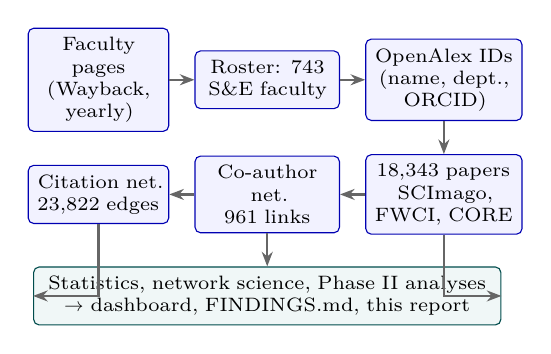
\begin{tikzpicture}[node distance=0.32cm, box/.style={rectangle, draw=blue!70!black, fill=blue!5, rounded corners=2pt, align=center, font=\scriptsize, minimum height=0.62cm},
  arrow/.style={-{Stealth[scale=0.8]}, thick, draw=gray!80!black}]
\node (a) [box, text width=1.55cm] {Faculty pages\\(Wayback, yearly)};
\node (b) [box, right=of a, text width=1.6cm] {Roster: \nFaculty{}\\S\&E faculty};
\node (c) [box, right=of b, text width=1.75cm] {OpenAlex IDs\\(name, dept., ORCID)};
\node (d) [box, below=0.42cm of c, text width=1.75cm] {\nPapers{} papers\\SCImago, FWCI, CORE};
\node (e) [box, left=of d, text width=1.6cm] {Co-author net.\\\nLinks{} links};
\node (f) [box, left=of e, text width=1.55cm] {Citation net.\\\nInternal{} edges};
\node (g) [box, below=0.42cm of e, text width=5.7cm, fill=teal!6, draw=teal!60!black] {Statistics, network science, Phase II analyses\\$\rightarrow$ dashboard, FINDINGS.md, this report};
\draw [arrow] (a) -- (b); \draw [arrow] (b) -- (c); \draw [arrow] (c) -- (d); \draw [arrow] (d) -- (e); \draw [arrow] (e) -- (f);
\draw [arrow] (e) -- (g); \draw [arrow] (f) |- (g); \draw [arrow] (d) |- (g);
\end{tikzpicture}
\caption{Pipeline from faculty pages to the analyses.}
\label{fig:pipeline}
\end{figure}

% ==============================================================================
\section{Methods}
\label{sec:methods}

\subsection{Bibliometric measures}
The \emph{field-weighted citation impact} of paper $p$ compares its citations $c_p$ with the world average for papers of the same field $f$, year $y$
and type $t$ (1 = world average):
\begin{equation}\label{eq:fwci}
\mathrm{FWCI}_p=\frac{c_p}{\bar{c}(f_p,y_p,t_p)}.
\end{equation}
A faculty member's h-index is the largest $h$ such that $h$ of their papers have at least $h$ citations each; we compute it from their 2016--2026
papers. The Q1 share is the number of papers in Q1 journals divided by the number of papers in journals with a SCImago quartile.

\subsection{Statistical tests}
Faculty-level medians are compared with the Mann--Whitney test and shares with the $\chi^2$ test. To compare the institutes fairly we fit, for every
paper,
\begin{equation}\label{eq:reg}
\log(1+\mathrm{FWCI}_p)=\beta_0+\beta_S\,\mathbb{1}[p\in S]+\boldsymbol{\gamma}^{\top}\mathbf{x}_p+\varepsilon_p ,
\end{equation}
where $\mathbf{x}_p$ holds branch, year, collaboration type, venue type and team size; the Surathkal effect is $100(e^{\beta_S}-1)\%$, with errors
robust and also clustered by faculty member. Branch gaps use bootstrap 95\% intervals (2.5th and 97.5th percentiles of 2{,}000 resamples), and the
$m$ branch $p$-values are corrected with Benjamini--Hochberg, $p^{adj}_{(i)}=\min_{j\geq i}\, m\,p_{(j)}/j$. Rank correlations use Spearman's
\begin{equation}\label{eq:spearman}
\rho=1-\frac{6\sum_i d_i^2}{n(n^2-1)},
\end{equation}
with an exact $p$-value from all $n!$ orderings when $n$ is small ($6!=720$ for six NITs).

\subsection{Network measures}
With adjacency matrix $A$, the degree is $k_i=\sum_j A_{ij}$. Betweenness counts the shortest paths through a node and PageRank (damping $d=0.85$)
ranks papers by the rank of the papers citing them:
\begin{equation}\label{eq:btw}
C_B(i)=\sum_{s\neq i\neq t}\frac{\sigma_{st}(i)}{\sigma_{st}},\qquad PR(v)=\frac{1-d}{N}+d\!\sum_{u\to v}\frac{PR(u)}{k_{out}(u)},
\end{equation}
where $\sigma_{st}$ is the number of shortest $s$--$t$ paths and $\sigma_{st}(i)$ those through $i$. The local clustering is
$C_i=2T_i/[k_i(k_i-1)]$ ($T_i$ triangles through $i$), $C$ its average, and $L$ the mean shortest-path length. Against random graphs with the same
degrees ($C_r$, $L_r$) the small-world index is
\begin{equation}\label{eq:sigma}
\sigma=\frac{C/C_r}{L/L_r},
\end{equation}
with $\sigma\gg1$ meaning a small world. Degree assortativity is the Pearson correlation of the degrees at the two ends of an edge~\cite{newman2002},
\begin{equation}\label{eq:assort}
r=\frac{\sum_{jk}jk\,(e_{jk}-q_jq_k)}{\sigma_q^{2}},
\end{equation}
where $e_{jk}$ is the share of edges joining remaining degrees $j$ and $k$ and $q_k$ its marginal; $r>0$ means hubs link to hubs. Communities
maximise the Louvain modularity
\begin{equation}\label{eq:mod}
Q=\frac{1}{2m}\sum_{ij}\Big(A_{ij}-\frac{k_ik_j}{2m}\Big)\delta(c_i,c_j),
\end{equation}
and are compared with departments by the normalised mutual information $\mathrm{NMI}=2I(X;Y)/[H(X)+H(Y)]$. The rich-club coefficient
$\phi(k)=2E_{>k}/[N_{>k}(N_{>k}-1)]$ is divided by its value in rewired graphs, $\rho(k)=\phi/\phi_{rand}$. Degree distributions are fitted with a
power law $p(k)\propto k^{-\alpha}$ ($k\geq k_{min}$) and a log-normal, compared by a likelihood-ratio test.

\subsection{Growth and link prediction}
The densification law~\cite{leskovec2005} relates links $E$ and connected faculty $N$ over the years,
\begin{equation}\label{eq:dens}
E(t)\propto N(t)^{a},\qquad \langle k\rangle=\frac{2E}{N}\propto N^{a-1},
\end{equation}
so $a>1$ means the average degree grows; the effective diameter is the distance within which 90\% of connected pairs lie. Preferential attachment is
measured by the kernel $\mathbb{E}[\Delta k_i]\propto k_i^{\,\alpha}$ ($\alpha=1$: linear). For link prediction every unlinked pair $(x,y)$ gets
the features common neighbours $|\Gamma(x)\cap\Gamma(y)|$, Adamic--Adar $\sum_{z\in\Gamma(x)\cap\Gamma(y)}1/\log k_z$, resource allocation
$\sum_z 1/k_z$, Jaccard $|\Gamma(x)\cap\Gamma(y)|/|\Gamma(x)\cup\Gamma(y)|$, preferential attachment $k_xk_y$, output, and same department / NIT,
and a logistic regression gives
\begin{equation}\label{eq:logit}
P(x\sim y)=\frac{1}{1+e^{-\mathbf{w}^{\top}\mathbf{f}_{xy}}}.
\end{equation}
We report the AUC (the chance that a real new pair is ranked above a non-pair), the number of correct pairs in the top $K$, and the lift
(precision at $K$ divided by the base rate).

\subsection{Spreading and synchronisation}
In the SIR model each infected faculty member passes an idea once along each link with probability $\beta$. The take-off threshold can be estimated
from the degrees (mean field), from the adjacency spectrum, or, correctly for SIR, from the non-backtracking matrix $B$~\cite{karrer2014}:
\begin{equation}\label{eq:sir}
\beta_c^{MF}=\frac{\langle k\rangle}{\langle k^2\rangle-\langle k\rangle},\qquad
\beta_c^{(1)}=\frac{1}{\lambda_1},\qquad \beta_c=\frac{1}{\lambda_{NB}},
\end{equation}
with $B_{(i\to j),(k\to l)}=\delta_{jk}(1-\delta_{il})$ and $1/\lambda_1$ a lower bound. In the Kuramoto model each faculty member is an
oscillator with natural frequency $\omega_i\sim N(0,1)$,
\begin{equation}\label{eq:kur}
\frac{d\theta_i}{dt}=\omega_i+K\sum_jA_{ij}\sin(\theta_j-\theta_i),\qquad re^{i\psi}=\frac{1}{N}\sum_je^{i\theta_j},
\end{equation}
and partial synchrony ($r$ rising) starts at~\cite{restrepo2005}
\begin{equation}\label{eq:kc}
K_c=\frac{K_0}{\lambda_1},\qquad K_0=\frac{2}{\pi g(0)}\approx1.596 .
\end{equation}
How easily the whole network locks is measured by the Laplacian eigenratio $\mu_N/\mu_2$ of $L=D-A$ (smaller = easier). For Indian partners
we fit the gravity model $\log(\text{papers}_{ij})=c+\beta\log(\text{size}_j)-\delta\log(\text{distance}_{ij})$.

% ==============================================================================
\section{Publication Statistics}
\label{sec:stats}

\begin{figure}[!tbp]
\centering
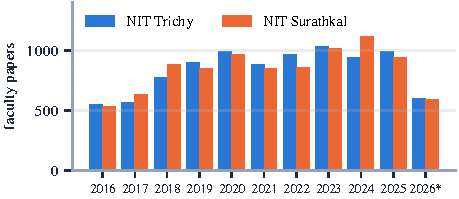
\includegraphics[width=\columnwidth]{figures/fig_trend.pdf}
\caption{Faculty papers per year (*2026 = January to mid-October). A joint paper counts for both NITs.}
\label{fig:trend}
\end{figure}

\subsection{Trend and head-to-head}
Output grew \growth$\times$, from \yrA{} papers in 2016 to \yrB{} in 2025, and the two NITs are level every year (Fig.~\ref{fig:trend}).
Table~\ref{tab:h2h} compares them. NIT Trichy papers collect more raw citations (\citT{} vs \citS{} per paper), but raw counts are not
field-normalised: in model~(\ref{eq:reg}) Surathkal is \fwciEffect\% ($p=\pRobust$; $p=\pClust$ with errors clustered by faculty), i.e.\
\textbf{no significant difference in impact}. Surathkal faculty publish more each, but much of this is rank mix: \asstT{} of Trichy's faculty are
Assistant Professors against \asstS, and the gap falls from \gapRaw{} to \gapRank{} for people of the same rank (Professors publish the same,
$p=\pProf$).

\begin{table}[!tbp]
\centering\small
\caption{Head-to-head. Bold = significantly higher (Mann--Whitney or $\chi^2$, $p<0.05$).}
\label{tab:h2h}
\begin{tabular}{@{}lrr@{}}
\toprule
 & Trichy & Surathkal \\
\midrule
Faculty (regular, S\&E, incl.\ former) & 415 & 328 \\
Papers 2016--2026 & 9{,}184 & 9{,}206 \\
Share in journals & 80\% & 68\% \\
Citations per paper (raw) & 15.2 & 13.6 \\
Mean / median FWCI & 1.31 / 0.63 & 1.39 / 0.65 \\
Top 10\% cited (world) & 13.6\% & 14.3\% \\
Q1 share of ranked journal papers & 35.2\% & \textbf{38.3\%} \\
Share in IF $>$ 5 journals & 33.0\% & 33.8\% \\
Median papers per faculty & 19 & \textbf{31} \\
Median h-index (2016--2026) & 7 & \textbf{9} \\
\bottomrule
\end{tabular}

\end{table}

\subsection{Journal quality and top journals}
More than a third of the ranked journal papers are Q1: \qOneT{} at Trichy and \qOneS{} at Surathkal ($\chi^2$, $p<0.001$; Fig.~\ref{fig:quart}). The
share in journals with IF $>5$ is level (\ifFiveT{} vs \ifFiveS; IF is OpenAlex's 2-year mean citedness). Both NITs publish most in the same venues
(Table~\ref{tab:journals}).

\begin{figure}[!tbp]
\centering
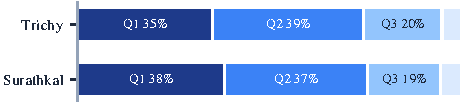
\includegraphics[width=\columnwidth]{figures/fig_quartiles.pdf}
\caption{Ranked journal papers by SCImago quartile.}
\label{fig:quart}
\end{figure}

\begin{table}[!tbp]
\centering\scriptsize
\caption{Top 5 journals of each NIT (papers, most common SCImago quartile, median IF).}
\label{tab:journals}
\begin{tabular}{@{}lrcr@{}}
\toprule
Journal & Papers & Q & IF \\
\midrule
\multicolumn{4}{@{}l}{\textit{NIT Trichy}} \\
Materials Today Proceedings & 288 & -- & 5.1 \\
Transactions of the Indian Institute of Met\ldots{} & 92 & Q3 & 2.0 \\
Journal of Materials Engineering and Perfor\ldots{} & 78 & Q2 & 2.0 \\
Materials Research Express & 61 & Q3 & 3.0 \\
Journal of Alloys and Compounds & 61 & Q1 & 6.4 \\
\midrule
\multicolumn{4}{@{}l}{\textit{NIT Surathkal}} \\
Materials Today Proceedings & 230 & -- & 5.1 \\
IEEE Access & 111 & Q1 & 6.5 \\
Journal of Materials Engineering and Perfor\ldots{} & 77 & Q2 & 2.0 \\
Materials Research Express & 76 & Q3 & 3.0 \\
Journal of Alloys and Compounds & 49 & Q1 & 6.4 \\
\bottomrule
\end{tabular}

\end{table}

\subsection{Faculty h-index}
Fig.~\ref{fig:hindex} shows the h-index of each faculty member computed from their 2016--2026 papers. The median is \hT{} at Trichy and \hS{} at
Surathkal ($p=\pH$), and the median number of papers is \papMedT{} vs \papMedS{} ($p<0.001$), while mean FWCI per person does not differ
($p=\pFwciPers$). Trichy's larger 0--4 bar fits with its many recently hired Assistant Professors. At the individual level we rank the \nRanked{} current faculty with at
least \rankMin{} papers by a composite score (the mean percentile of papers, citations, h-index, mean FWCI, top-10\%-cited papers and Q1 or CORE
A*/A papers); weighting quality more changes little (Spearman \rankRho). Table~\ref{tab:faculty} gives the top five of each NIT.

\begin{table}[!tbp]
\centering\scriptsize\setlength{\tabcolsep}{3.5pt}
\caption{Faculty level: top five of each NIT by the composite research score (overall rank among both NITs; $h$ and FWCI from 2016--2026 papers).}
\label{tab:faculty}
\begin{tabular}{@{}rllrrrrr@{}}
\toprule
Rank & Faculty member & Dept. & Papers & Cites & $h$ & FWCI & Score \\
\midrule
\multicolumn{8}{@{}l}{\textit{NIT Trichy}} \\
2 & S Suresh & Mechanical & 156 & 4{,}579 & 39 & 2.13 & 98.0 \\
6 & A Chandra Bose & Physics & 98 & 3{,}132 & 31 & 2.21 & 96.1 \\
7 & P Sivashanmugam & Chemical & 77 & 3{,}298 & 31 & 2.42 & 95.8 \\
9 & R Karvembu & Chemistry & 145 & 4{,}126 & 38 & 1.67 & 95.4 \\
10 & G Arthanareeswaran & Chemical & 171 & 4{,}194 & 35 & 1.52 & 95.0 \\
\multicolumn{8}{@{}l}{\textit{NIT Surathkal}} \\
1 & Ramesh M R & Mechanical & 180 & 4{,}129 & 39 & 2.41 & 98.5 \\
3 & Denthaje Krishna Bhat & Chemistry & 98 & 4{,}904 & 48 & 2.33 & 97.8 \\
4 & Bibhuti Bhusan Das & Civil & 123 & 2{,}398 & 26 & 3.68 & 97.3 \\
5 & Arun Mohan Isloor & Chemistry & 87 & 2{,}744 & 30 & 2.36 & 96.6 \\
8 & Jeyaraj P & Mechanical & 130 & 2{,}448 & 27 & 1.86 & 95.6 \\
\bottomrule
\end{tabular}

\end{table}

\begin{figure}[!tbp]
\centering
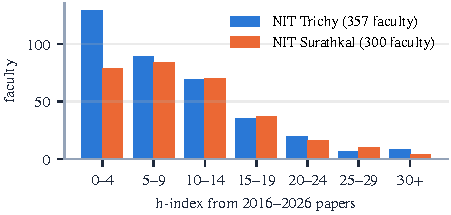
\includegraphics[width=\columnwidth]{figures/fig_hindex.pdf}
\caption{h-index distribution (faculty with at least one paper).}
\label{fig:hindex}
\end{figure}

\subsection{Research areas and AI}
Engineering is about half of each NIT's papers, followed by computer science and materials science (Table~\ref{tab:fields}). Surathkal has
relatively more computer science and mathematics, Trichy more materials, energy and chemistry. AI is spreading (Fig.~\ref{fig:ai}): AI papers rose
from \aiA\% of all papers in 2016 to \aiB\% in 2025 (\aiOA\% $\to$ \aiOB\% outside the computing departments), and \aiDeptB{} of \aiDeptN{} departments
now have at least 5\% AI papers (\aiDeptA{} in 2016--18). The work we build on is getting more recent: the Price index (share of references at most
five years old) rose from about \priceA\% in \priceYA{} to \priceB\% in \priceYB{} (Fig.~\ref{fig:recency}; \priceAll\% overall), and papers that
cite more recent work have slightly higher FWCI (Spearman \priceRho{} within departments).

\begin{figure}[!tbp]
\centering
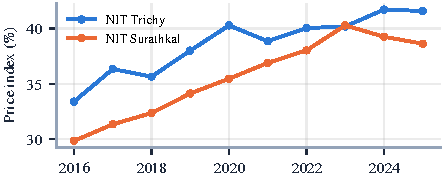
\includegraphics[width=\columnwidth]{figures/fig_recency.pdf}
\caption{Price index: share of each year's references that are at most five years old.}
\label{fig:recency}
\end{figure}

\begin{table}[!tbp]
\centering\scriptsize
\caption{Papers by OpenAlex field (a paper counts once per NIT).}
\label{tab:fields}
\begin{tabular}{@{}lrrrr@{}}
\toprule
Field (OpenAlex) & \multicolumn{2}{c}{Trichy} & \multicolumn{2}{c}{Surathkal} \\
\midrule
Engineering & 4{,}524 & 49\% & 4{,}526 & 49\% \\
Computer Science & 1{,}444 & 16\% & 1{,}639 & 18\% \\
Materials Science & 1{,}023 & 11\% & 854 & 9\% \\
Environmental Science & 514 & 6\% & 585 & 6\% \\
Energy & 454 & 5\% & 274 & 3\% \\
Mathematics & 156 & 2\% & 316 & 3\% \\
Chemistry & 264 & 3\% & 170 & 2\% \\
All other fields & 804 & 9\% & 842 & 9\% \\
\bottomrule
\end{tabular}

\end{table}

\begin{figure}[!tbp]
\centering
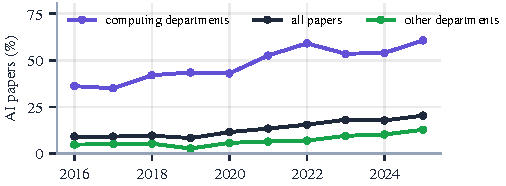
\includegraphics[width=\columnwidth]{figures/fig_ai.pdf}
\caption{Share of AI papers per year (2026 left out).}
\label{fig:ai}
\end{figure}

\subsection{Department level}
FWCI differs much more between branches than between the two NITs (Fig.~\ref{fig:branches}, Table~\ref{tab:branches}). After the
Benjamini--Hochberg correction over the \nBranch{} branches, Surathkal is clearly stronger in \brS{} and Trichy in \brT; Mechanical and ECE differ only
before the correction, and the other branches are level. An institute-level ``winner'' hides this picture.

\begin{figure}[!tbp]
\centering
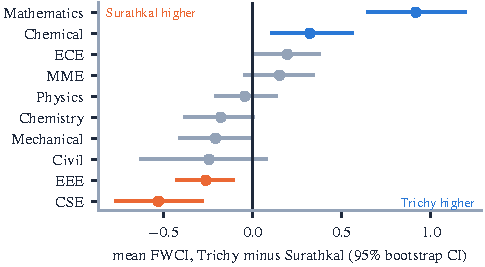
\includegraphics[width=\columnwidth]{figures/fig_branches.pdf}
\caption{Mean FWCI gap by branch with 95\% bootstrap intervals; coloured = significant after correction.}
\label{fig:branches}
\end{figure}

\begin{table}[!tbp]
\centering\scriptsize
\caption{Department level: papers and mean FWCI by branch ($p_{adj}$ = Benjamini--Hochberg; bold = significant after correction, $\dagger$ = only before it).}
\label{tab:branches}
\begin{tabular}{@{}lrrrrrl@{}}
\toprule
Branch & \multicolumn{2}{c}{Papers} & \multicolumn{2}{c}{Mean FWCI} & $p_{adj}$ & Stronger \\
\cmidrule(lr){2-3}\cmidrule(lr){4-5}
 & T & S & T & S & & \\
\midrule
CSE & 701 & 968 & 1.00 & 1.53 & 0.000 & \textbf{Surathkal} \\
EEE & 851 & 816 & 0.97 & 1.23 & 0.004 & \textbf{Surathkal} \\
Civil & 754 & 992 & 1.69 & 1.94 & 0.186 & level \\
Mechanical & 731 & 1{,}715 & 1.43 & 1.63 & 0.064 & Surathkal$^\dagger$ \\
Chemistry & 739 & 758 & 1.33 & 1.51 & 0.098 & level \\
Physics & 771 & 374 & 1.03 & 1.07 & 0.617 & level \\
MME & 551 & 514 & 1.13 & 0.98 & 0.143 & level \\
ECE & 1{,}114 & 797 & 1.18 & 0.98 & 0.064 & Trichy$^\dagger$ \\
Chemical & 651 & 388 & 1.59 & 1.27 & 0.012 & \textbf{Trichy} \\
Mathematics & 296 & 500 & 1.48 & 0.56 & 0.000 & \textbf{Trichy} \\
\bottomrule
\end{tabular}

\end{table}

\begin{table*}[!tp]
\centering\scriptsize
\caption{The ten most-cited papers (citations as of 7 October 2026; FWCI 1 = world average). T = NIT Trichy, S = NIT Surathkal.}
\label{tab:cited}
\begin{tabular}{@{}rp{8.6cm}p{3.7cm}rrrc@{}}
\toprule
\# & Title & Journal & Year & Citations & FWCI & NIT \\
\midrule
1 & A Review of Classical and Nonclassical Nucleation Theories & Crystal Growth \& Design & 2016 & 877 & 19.5 & T \\
2 & Lignocellulosic biomass-based pyrolysis: A comprehensive review & Chemosphere & 2021 & 536 & 25.7 & T \\
3 & Crop pest classification based on deep convolutional neural network and transfer\ldots{} & Computers and Electronics in Agr\ldots{} & 2019 & 514 & 28.7 & T \\
4 & Characterization of raw and alkali treated new natural cellulosic fibers from Tri\ldots{} & International Journal of Biologi\ldots{} & 2018 & 474 & 18.4 & T \\
5 & A review on composite materials and process parameters optimisation for the fused\ldots{} & Virtual and Physical Prototyping & 2017 & 457 & 22.4 & T \\
6 & Influence of wood dust fillers on the mechanical, thermal, water absorption and b\ldots{} & Journal of Polymer Research & 2019 & 456 & 13.3 & T \\
7 & Are lead-free relaxor ferroelectric materials the most promising candidates for e\ldots{} & Progress in Materials Science & 2022 & 426 & 20.7 & T \\
8 & Green synthesis of iron nanoparticles using different leaf extracts for treatment\ldots{} & Journal of Cleaner Production & 2016 & 408 & 11.9 & S \\
9 & Application of life cycle assessment in municipal solid waste management: A world\ldots{} & Journal of Cleaner Production & 2018 & 392 & 32.4 & S \\
10 & Enhancement of the properties of fly ash based geopolymer paste by incorporating\ldots{} & Construction and Building Materi\ldots{} & 2017 & 385 & 23.2 & S \\
\bottomrule
\end{tabular}

\end{table*}

\subsection{Most-cited papers}
Table~\ref{tab:cited} lists the ten most-cited papers: \topTrichy{} are from NIT Trichy and \topReview{} have ``review'' in the title.

% ==============================================================================
\section{Citation Network}
\label{sec:citation}
\textbf{PageRank.} Table~\ref{tab:pagerank} gives the top 10 papers by PageRank~(\ref{eq:btw}). They must be read with care: \selfShare{} of the
citations between our papers share an author, and without them none of these ten stays in the top 10, so the list mainly shows groups building on
their own earlier work.

\textbf{In-degree.} \zeroIndeg{} of our papers are never cited by another of our papers; $k_{in}$ is heavy-tailed (maximum \maxIndeg,
Fig.~\ref{fig:degrees}b) and a log-normal fits it better than a power law ($\alpha\approx\alphaIn$).

\begin{table}[!tbp]
\centering\scriptsize
\caption{Top 10 papers by PageRank in the internal citation network ($k_{in}$ = cited by our papers).}
\label{tab:pagerank}
\begin{tabular}{@{}rp{5.15cm}crr@{}}
\toprule
\# & Title & NIT & Year & $k_{in}$ \\
\midrule
1 & Effect of particle surface treatment and bl\ldots{} & S & 2016 & 33 \\
2 & Myo-inositol based nano-PCM for solar therm\ldots{} & T & 2016 & 15 \\
3 & Studies on the weldability, mechanical prop\ldots{} & T & 2018 & 17 \\
4 & Printability of multiwalled SS 316L by wire\ldots{} & T & 2019 & 6 \\
5 & Half-sandwich RuCl 2 ($\eta$ 6 -p-cymene) core c\ldots{} & T & 2016 & 40 \\
6 & Investigating the contrast diurnal relation\ldots{} & T & 2022 & 21 \\
7 & High Thermoelectric Performance of Co-Doped\ldots{} & S & 2017 & 29 \\
8 & Experimental investigation on the mechanica\ldots{} & T & 2016 & 9 \\
9 & Effect of Oxide Fluxes on Depth of Penetrat\ldots{} & T & 2016 & 2 \\
10 & Hydrothermally Synthesized h-MoO 3 and $\alpha$-Mo\ldots{} & T & 2016 & 7 \\
\bottomrule
\end{tabular}

\end{table}

\begin{figure}[!tbp]
\centering
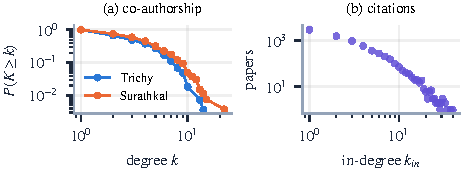
\includegraphics[width=\columnwidth]{figures/fig_degrees.pdf}
\caption{(a) Co-authorship degree, complementary cumulative distribution; (b) citation in-degree distribution (log--log).}
\label{fig:degrees}
\end{figure}

\textbf{Flow between institutes.} With other Indian institutes, Trichy received \flowRT{} citations and gave \flowGT{} (ratio \ratioT); Surathkal
received \flowRS{} and gave \flowGS{} (\ratioS). The totals are below 1 because of the early years, when our papers had little time to be cited;
since 2023 both NITs receive more than they give every year (ratio \flowLateMin--\flowLateMax, Fig.~\ref{fig:flow}). There is a clear hierarchy:
IITs give back \cIIT{} citations and CSIR labs \cCSIR{} per citation we give them, while universities and colleges cite us more than we cite them
(\cUni). Between the two NITs, Trichy papers cite Surathkal papers \citeTS{} times and the reverse \citeST{} times.

\begin{figure}[!tbp]
\centering
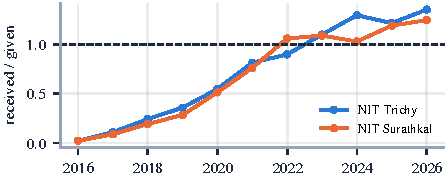
\includegraphics[width=\columnwidth]{figures/fig_flow.pdf}
\caption{Citations received from other Indian institutes per citation given to them, by year.}
\label{fig:flow}
\end{figure}

% ==============================================================================
\section{Authorship Network}
\label{sec:authorship}
\nConn{} of the \nNodes{} faculty have a faculty co-author; the largest connected group has \nLCC{} faculty, and only \nCross{} links (\crossPct)
join the two NITs. \textbf{Degree and betweenness.} The degree is heavy-tailed (maximum \maxDeg, Fig.~\ref{fig:degrees}a), and a log-normal again
beats a power law. Betweenness~(\ref{eq:btw}) picks out the bridges between departments (Table~\ref{tab:central}); removing the 10 main bridges
disconnects \bridgeT{} (Trichy) and \bridgeS{} (Surathkal) of connected faculty pairs, against \randT{} and \randS{} for 10 random faculty.

\begin{table}[!tbp]
\centering\scriptsize
\caption{Faculty with the highest betweenness $C_B$ (normalised); $k$ = faculty co-authors.}
\label{tab:central}
\begin{tabular}{@{}llcrr@{}}
\toprule
Faculty member & Dept. & NIT & $k$ & $C_B$ \\
\midrule
Ramesh M R & Mechanical & S & 22 & 0.100 \\
P Palanisamy & ECE & T & 10 & 0.077 \\
Gangadharan K V & Mechanical & S & 14 & 0.071 \\
N Sivakumaran & ICE & T & 13 & 0.060 \\
Jeny Rajan & CSE & S & 10 & 0.060 \\
B Venkatesa Perumal & EEE & S & 7 & 0.059 \\
\bottomrule
\end{tabular}

\end{table}

\begin{figure}[!tbp]
\centering
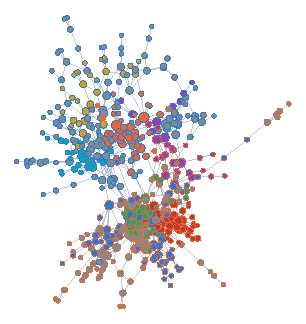
\includegraphics[width=\columnwidth]{figures/fig_coauthor.pdf}
\caption{Largest connected group of the faculty co-authorship network (\nLCC{} faculty; spring layout). Fill colour = the ten largest Louvain communities (grey = smaller ones), ring = NIT (blue Trichy, orange Surathkal), size = degree.}
\label{fig:coauthor}
\end{figure}

\textbf{Communities.} Louvain~(\ref{eq:mod}) finds \nComm{} communities among the connected faculty ($Q=\modQ$, \commTen{} with 10 or more members;
Fig.~\ref{fig:coauthor}). They follow departments closely (NMI \nmi{} vs \nmiRand{} for random labels; branch assortativity \assortBranch).

\textbf{Small world and mixing.} The average path length is $L=\apl$ (random graphs with the same degrees: \aplR) and the clustering is $C=\clust$
vs \clustR, so $\sigma=\swSigma\gg1$ in~(\ref{eq:sigma}): a small world. Hubs work with hubs: $r=\assortDeg$ in~(\ref{eq:assort}) against
\assortNull{} in rewired copies ($z=\assortZ$), and $k_{nn}(k)$ rises with $k$ (Fig.~\ref{fig:knn}). Rank mixing is weak but above chance
($r=\assortRank$, $z=\zRank$), and the 10 best-connected faculty co-author with each other \rcRho$\times$ more than chance (rich club; mostly one
Surathkal Mechanical and MME group).

\begin{figure}[!tbp]
\centering
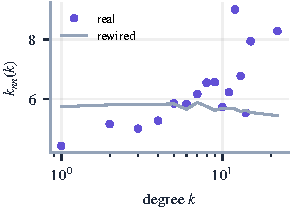
\includegraphics[width=0.62\columnwidth]{figures/fig_knn.pdf}
\caption{Average neighbour degree $k_{nn}(k)$, real network vs degree-preserving rewired copies.}
\label{fig:knn}
\end{figure}

% ==============================================================================
\section{Indian Connections}
\label{sec:indian}
Both NITs co-author widely within India: Trichy has joint papers with \partT{} Indian institutes and Surathkal with \partS{}
(Table~\ref{tab:partners}); \indCollT{} and \indCollS{} of their papers have an Indian partner and \forCollT{} and \forCollS{} a foreign one.
Universities and colleges account for \uniShare{} of the joint papers, mostly nearby ones: \geoJoint\% of joint papers but only \geoCite\% of
citations are within 300\,km (Fig.~\ref{fig:geo}). In the gravity model the distance exponent is $\delta=\gravJ$ for joint papers but only \gravC{} for
citations: doubling the distance cuts joint papers by \geoElJ\% and citations by \geoElC\%. Working together needs closeness; reading each other's work
does not.

\begin{table}[!tbp]
\centering\scriptsize
\caption{Largest Indian co-authorship partners (joint papers 2016--2026; ``cites us'' = their citations to our papers).}
\label{tab:partners}
\begin{tabular}{@{}clp{1.65cm}rr@{}}
\toprule
NIT & Partner institute & Type & Joint & Cites us \\
\midrule
T & Vellore Institute of Technolo\ldots{} & University &216 & 1{,}953 \\
T & SRM Institute of Science and\ldots{} & University &155 & 1{,}648 \\
T & Indian Institute of Technolog\ldots{} & IIT &119 & 527 \\
T & Bharathidasan University & University &109 & 319 \\
S & Manipal Academy of Higher Edu\ldots{} & University &461 & 898 \\
S & Vellore Institute of Technolo\ldots{} & University &158 & 1{,}388 \\
S & Indian Institute of Science B\ldots{} & IISER / IISc &126 & 569 \\
S & Nitte University & University &114 & 252 \\
\bottomrule
\end{tabular}

\end{table}

\begin{figure}[!tbp]
\centering
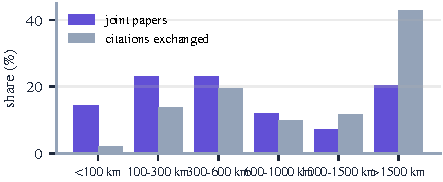
\includegraphics[width=\columnwidth]{figures/fig_geo.pdf}
\caption{Share of joint papers and of citations exchanged with Indian partners, by distance.}
\label{fig:geo}
\end{figure}

% ==============================================================================
\section{Phase II: Growth, Prediction and Dynamics}
\label{sec:phase2}

\begin{figure*}[!tp]
\centering
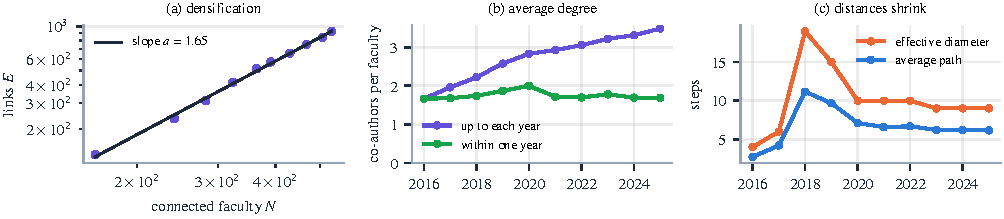
\includegraphics[width=\textwidth]{figures/fig_growth.pdf}
\caption{Growth of the faculty co-authorship network, 2016--2025: (a) densification, links against connected faculty on log--log axes with the fitted exponent $a$; (b) average number of faculty co-authors, counting all links so far and only that year's; (c) effective diameter and average path length of the largest group.}
\label{fig:growth}
\end{figure*}

\subsection{Densification and shrinking distances}
The links follow the densification law~(\ref{eq:dens}) with $a=\aExp$ ($R^2=\aRsq$; Fig.~\ref{fig:growth}a). So the average number of faculty
co-authors rose from \degA{} to \degB{} (2016$\to$2025), although within any one year a faculty member writes with only \yrDegMin--\yrDegMax{}
colleagues (Fig.~\ref{fig:growth}b): old links stay while new ones are added. Distances shrink (Fig.~\ref{fig:growth}c): the effective diameter fell
from \diamPeak{} steps in \diamYear, when the giant group formed through thin bridges, to \diamNow, and the average path from \aplPeak{} to \apl.
Real growing networks give $a$ between 1.08 and 1.68 and also show shrinking diameters~\cite{leskovec2005}, so our values are normal.

\begin{figure*}[!tp]
\centering
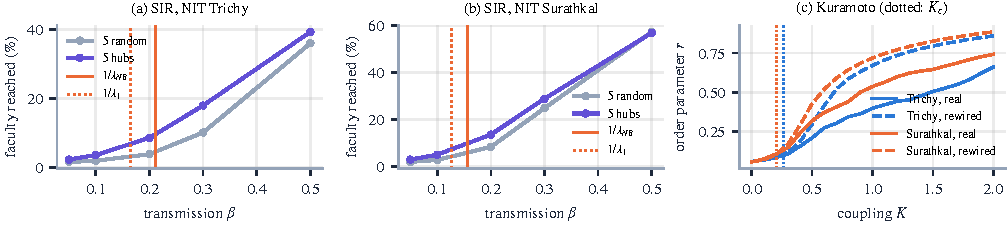
\includegraphics[width=\textwidth]{figures/fig_dynamics.pdf}
\caption{Theory against simulation. (a, b) SIR: share of faculty reached from 5 random starters or the 5 biggest hubs (mean of 500 runs), with the thresholds $1/\lambda_{NB}$ (solid) and $1/\lambda_1$ (dotted) of~(\ref{eq:sir}). (c) Kuramoto order parameter $r$ for the real networks and rewired copies, with $K_c$ of~(\ref{eq:kc}) (dotted).}
\label{fig:dyn}
\end{figure*}

\subsection{Rich get richer, and team size}
New faculty co-authors grow only weakly with current ones (Fig.~\ref{fig:kernelteam}a): faculty with 9 or more gain \kerNine{} a year against
\kerOne{} for those with one, a kernel exponent $\alpha=\kerA$ (Trichy \kerT, Surathkal \kerS), well below the linear $\alpha=1$ and below the
0.75--0.8 measured for co-authorship networks~\cite{barabasi2002}. Citations show a stronger effect ($\alpha=\richA$). Impact rises steadily with team
size (Fig.~\ref{fig:kernelteam}b), from \teamA{} for single authors to \teamB{} for 10--19 authors; only \teamBig{} faculty paper has 20 or more authors.

\begin{figure}[!tbp]
\centering
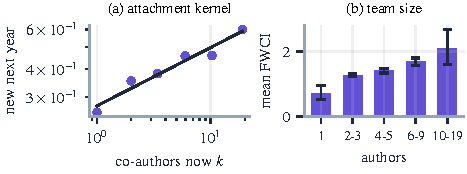
\includegraphics[width=\columnwidth]{figures/fig_kernel_team.pdf}
\caption{(a) New faculty co-authors next year against current ones (log--log, fitted line); (b) mean FWCI by number of authors with 95\% intervals.}
\label{fig:kernelteam}
\end{figure}

\subsection{Predicting new collaborations}
The model~(\ref{eq:logit}) is \textbf{trained once on 2016--2022} (windows $t\to t+1$) and given only the 2022 network. It then predicts the first
joint papers of 2023, 2024 and 2025 \emph{without seeing any later data}. It ranks the real new pairs well (AUC \lpAUC), but only about \lpBase\% of
candidate pairs start working together each year, so exact hits are rare (Table~\ref{tab:lp}). Its top 1\% holds \lpTop{} real new pairs,
\lpLiftMin--\lpLiftMax$\times$ better than a random list (Fig.~\ref{fig:lp}); all \lpMatches{} correct matches are same-department pairs and are listed
with the DOI of the first joint paper on the dashboard. \lpOut\% of 2025's new pairs involve faculty with no paper by 2022, which a fixed model cannot
see; a model re-trained every year finds more. Real co-authorship networks show the same low raw precision~\cite{libennowell2007}.

\begin{table}[!tbp]
\centering\scriptsize
\caption{Link prediction: fixed model trained on 2016--2022 and an updated model re-trained every year.}
\label{tab:lp}
\begin{tabular}{@{}lrrr@{}}
\toprule
 & 2023 & 2024 & 2025 \\
\midrule
Real new faculty pairs (reachable in 2022) & 95 (85) & 88 (68) & 84 (61) \\
\textbf{Fixed model}: AUC & \textbf{0.90} & \textbf{0.87} & \textbf{0.90} \\
\quad correct pairs in top 100 & 3 & 2 & 0 \\
\quad correct pairs in top 1\% ($\approx$1{,}570) & \textbf{19} (22$\times$) & \textbf{14} (21$\times$) & \textbf{9} (15$\times$) \\
Updated model: correct in top 1\% & 19 & 15 & 16 \\
\bottomrule
\end{tabular}

\end{table}

\begin{figure}[!tbp]
\centering
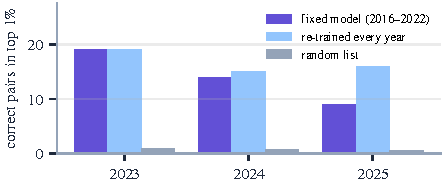
\includegraphics[width=\columnwidth]{figures/fig_linkpred.pdf}
\caption{Correct new pairs in the top 1\% of predicted pairs, against a random list of the same size.}
\label{fig:lp}
\end{figure}

\begin{table*}[!tp]
\centering\scriptsize
\caption{The six South Indian NITs, built the same way (NIRF 2025 faculty lists; self-cit.\ = share of citations between a NIT's own papers that share an author; $a$ = densification exponent).}
\label{tab:six}
\begin{tabular}{@{}lrrrrrrr@{}}
\toprule
NIT & Founded & Faculty & Asst.\ Prof. & Hired 21--25 & Papers/fac.\ 2024 & Self-cit. & $a$ \\
\midrule
Trichy & 1964 & 348 & 47\% & 21\% & 3.4 & 85\% & \textbf{1.41} \\
Surathkal & 1960 & 279 & 30\% & 9\% & 4.7 & 89\% & \textbf{1.74} \\
Warangal & 1959 & 327 & 35\% & 13\% & 4.2 & 87\% & \textbf{1.44} \\
Calicut & 1961 & 375 & 65\% & 35\% & 2.4 & 87\% & \textbf{1.39} \\
Puducherry & 2010 & 76 & 70\% & 62\% & 4.4 & 92\% & \textbf{1.31} \\
Andhra Pradesh & 2015 & 139 & 98\% & 68\% & 2.0 & 92\% & \textbf{1.19} \\
\bottomrule
\end{tabular}

\end{table*}

\subsection{Six South Indian NITs}
Table~\ref{tab:six} and Fig.~\ref{fig:six} compare all six South Indian NITs, built the same way (OpenAlex papers and each NIT's NIRF 2025 faculty
list; with our own faculty lists Trichy's $a$ is \aTrOwn{} and Surathkal's \aSuOwn). Every NIT densifies ($a=\aSixMin$--\aSixMax, close to the
real-network range), papers per head follow the rank mix, and \selfMin--\selfMax\% of citations between a NIT's own papers share an author everywhere.
NITs that hired more recently have lower exponents (Spearman~(\ref{eq:spearman}) $\rho=\rhoSix$, exact $p=\pSix$, $n=6$), but this is fragile: with a
second, independently cleaned dataset for Warangal and Calicut it weakens to $-0.60$ ($p=0.24$), and inside single NITs the link is not consistent.

\begin{figure}[!tbp]
\centering
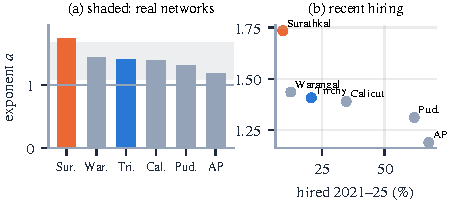
\includegraphics[width=\columnwidth]{figures/fig_six.pdf}
\caption{Six South Indian NITs: (a) densification exponent, shaded = range in real growing networks~\cite{leskovec2005}; (b) share hired in 2021--25 against $a$.}
\label{fig:six}
\end{figure}

\subsection{Other Phase II questions}
\begin{itemize}
\item \textbf{Students' own papers.} Papers with an NIT author but no faculty author add \stuN{} papers (\stuPct, \stuAll{} in all). Their median FWCI
equals the faculty median at Trichy (\stuMedT{} vs \facMedT) and is lower at Surathkal (\stuMedS{} vs \facMedS). Networks and rankings stay faculty-only.
\item \textbf{Who cites us.} Private universities cite us about as much as their size predicts (\privPer{} vs \pubPer{} citations per 1{,}000 of their
papers, $p=\privP$), but more of their citations come from people within three co-authorship steps of the cited authors (\privNear\% vs \pubNear\%),
i.e.\ former students and co-authors (Fig.~\ref{fig:citers}).
\item \textbf{Partners and impact.} A foreign co-author goes with \forEff\% FWCI for papers of the same field, year and team size, and foreign
universities \forUni\% (significant after correction), while IITs give \iitEff\% (not significant). The gain differs by country (Fig.~\ref{fig:countries}). This is an association, not a cause.
\item \textbf{Citation manipulation.} Only \manipShare{} of the \manipN{} Indian citations come from papers that cite 10 or more of ours, and the top-20
faculty ranking is unchanged without self-citations (Spearman \manipRho).
\end{itemize}

\subsection{Research questions on people, venues and data quality}
\begin{itemize}
\item \textbf{Inequality.} Citations are concentrated: the top 10\% of faculty hold \topTenC{} of all citations and the bottom half \botHalfC{}
(Gini \giniC{} for citations, \giniP{} for papers).
\item \textbf{Former faculty.} Of the \nFormer{} former faculty with papers, \movedIIT{} moved to IITs and \movedNIT{} to other NITs, mostly Assistant
Professors; as a group they were not weaker than those who stayed.
\item \textbf{Author roles.} Faculty are mostly last authors (supervisors): \asstLast{} of Assistant Professors' papers and \profLast{} of Professors',
while Assistant Professors are first author on only \asstFirst.
\item \textbf{Where to publish.} Against a Q1 journal paper of the same field and year, unranked conference papers have \confEff\% FWCI, Q2 journals
\qTwoEff\% and Q3--Q4 journals \qThreeEff\%, so a weak journal is not a better outlet than a conference.
\item \textbf{Open access.} \oaShare{} of papers are open; gold and green open access go with \oaGold\% and \oaGreen\% FWCI, diamond with \oaDiamond\%.
\item \textbf{Home citations.} \homeShare{} of the citations our papers receive come from our own two NITs; papers with more home references have
slightly higher FWCI (\homeEff\% per 10 points).
\item \textbf{Robustness.} Dropping the \nDoubt{} weakest author matches changes the paper count by \doubtPap\% and citations by \doubtCit\%; no
conclusion changes.
\end{itemize}

\begin{figure}[!tbp]
\centering
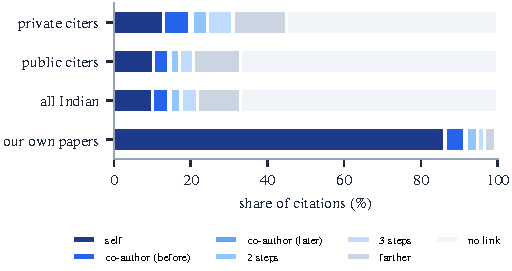
\includegraphics[width=\columnwidth]{figures/fig_citers.pdf}
\caption{How close citers are to the cited authors in the co-authorship network: the same person (self), an earlier or later co-author, or 2, 3 or more steps away.}
\label{fig:citers}
\end{figure}

\begin{figure}[!tbp]
\centering
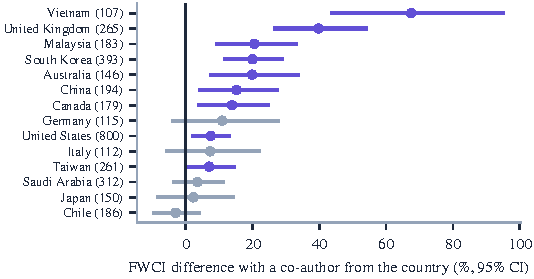
\includegraphics[width=\columnwidth]{figures/fig_countries.pdf}
\caption{FWCI difference for papers with a co-author from each country (countries with 100+ joint papers; grey = not significant).}
\label{fig:countries}
\end{figure}

\begin{table*}[!tp]
\centering\scriptsize\setlength{\tabcolsep}{4pt}\renewcommand{\arraystretch}{1.12}
\caption{Main findings, inferences and comparison with real networks or theory.}
\label{tab:findings}
\begin{tabular}{@{}p{2.5cm}p{4.4cm}p{4.5cm}p{5.4cm}@{}}
\toprule
Finding & Our numbers & What it means & Compared with real networks or theory \\
\midrule
\textbf{A small world: short paths and strong clustering} & average path 6.1 steps (random networks with the same degrees 4.5); average clustering 0.21 vs 0.011 (20$\times$ higher); transitivity 0.21 & Faculty sit in tight groups, yet a few links between groups keep everyone within a few steps. & Typical of co-authorship networks: in seven large ones the average distance is 4.0--9.7 and the clustering (transitivity) 0.072--0.726 (Newman 2001). Ours (6.1 and 0.21) falls inside both ranges. \\
\addlinespace[1.5pt]
\textbf{Well-connected faculty work with each other (assortative)} & degree assortativity r = 0.20 vs $-$0.02 in rewired networks (z = 6.9); by branch r = 0.66, by NIT r = 0.94, by rank only 0.07 & Hubs link to hubs, people stay in their branch and NIT, and rank matters little. & This is the usual pattern of social networks: co-authorship networks have r = 0.12--0.36, while technological and biological networks are disassortative (Newman 2002). \\
\addlinespace[1.5pt]
\textbf{No clean power law in the degree distributions} & a log-normal fits better than a power law for 4 of 4 degree and citation distributions (heavy tails, $\alpha$ $\approx$ 2.5--2.9) & A few people have many co-authors, but the network is not 'scale-free'. & Newman (2001) also found that collaboration networks are not pure power laws: their degree distributions have a cut-off. \\
\addlinespace[1.5pt]
\textbf{The network densifies: links grow faster than people} & links $\propto$ (connected faculty)$^{a}$ with a = 1.65 (R$^2$ = 0.998); the same exponent at the six South Indian NITs is 1.19--1.74 & Each faculty member gains co-authors over time, so the average number of co-authors keeps rising. & Real growing networks densify the same way, with a = 1.08--1.68 (citation graphs 1.56 and 1.68, US patents 1.66, internet routers 1.18, author--paper graphs 1.08--1.15; Leskovec et al. 2005). Ours and five of the six NITs are inside this range; Surathkal is just above it. \\
\addlinespace[1.5pt]
\textbf{Distances shrink as the network grows} & effective diameter 19 steps in 2018 $\to$ 9; average path in the largest group 11.2 $\to$ 6.1; co-authors per connected faculty member 1.67 $\to$ 3.48, but within any one year only 1.7--2.0 & The giant group formed in 2018 through thin bridges (long paths); new links then acted as shortcuts. People do not write with more colleagues each year; the totals rise because old links stay. & Leskovec et al. (2005) found shrinking diameters in real growing networks, largest when the giant component first appears; Barab\'asi et al. (2002) found that in co-authorship networks the separation falls and the average degree rises over time. \\
\addlinespace[1.5pt]
\textbf{Rich get richer: weak for collaborators, stronger for citations} & new faculty co-authors $\propto$ (current co-authors)$^{0.35}$ (Trichy 0.26, Surathkal 0.32); new citations $\propto$ (current citations)$^{0.75}$ & Well-connected faculty gain new collaborators only a little faster than others; highly cited papers gain citations much faster. & Barab\'asi et al. (2002) measured a stronger attachment for co-authorship, k$^{0.8}$ (mathematics) and k$^{0.75}$ (neuroscience). Our collaborator effect is weaker; our citation effect is close to theirs. \\
\addlinespace[1.5pt]
\textbf{New collaborations can be predicted, but exact hits are rare} & a model trained once on 2016--2022 and given only the 2022 network: AUC 0.90 / 0.87 / 0.90 for 2023, 2024, 2025; its top 1\% of pairs (about 1,569) holds 19 / 14 / 9 of the real new pairs, 15--22$\times$ better than random (42 correct matches listed) & Who will work together next is fairly predictable (same department, active people, common colleagues), but only about 1 candidate pair in 2,000 starts each year, so most predicted pairs do not happen yet. & Real co-authorship networks behave the same: a random prediction is right 0.15--0.48\% of the time and the best methods do up to about 55$\times$ better than random, with low raw precision (Liben-Nowell \& Kleinberg 2007). \\
\addlinespace[1.5pt]
\textbf{Ideas spread more easily at Surathkal, as the theory predicts} & SIR epidemic threshold $\beta_c$ = $1/\lambda_{NB}$ = 0.211 (Trichy) and 0.156 (Surathkal); simulated reach from 5 random starters at $\beta$ = 0.1 / 0.2 / 0.3: Trichy 1.9 / 3.9 / 10.1\%, Surathkal 2.8 / 8.4 / 24.8\% & Spreading takes off between $\beta$ = 0.2 and 0.3 at Trichy and around 0.15--0.2 at Surathkal, where the theory puts the thresholds; Surathkal's bigger, connected hubs raise $\lambda$ and so lower its threshold. & The threshold formula for SIR on real networks is the non-backtracking one (Karrer, Newman \& Zdeborov\'a 2014); worked out step by step in our PDF. \\
\addlinespace[1.5pt]
\textbf{Synchrony starts where theory says, but full synchrony is hard} & onset $K_c$ = $K_0/\lambda_1$ = 0.264 (Trichy) and 0.203 (Surathkal); simulated order parameter r at K = 0.2 / 0.3 / 0.4: Trichy 0.08 / 0.11 / 0.16, Surathkal 0.11 / 0.15 / 0.24 (noise level about 0.06); Laplacian eigenratio 670 vs 130 in rewired networks & Partial synchrony begins as predicted, but groups are joined by thin bridges, so the whole network is about 5$\times$ harder to bring into one rhythm than a random one. & The onset formula is Restrepo, Ott \& Hunt (2005); details in our PDF. \\
\addlinespace[1.5pt]
\textbf{Most citations between our own papers are self-citations, at every NIT} & 86\% of the 23,822 citations between our papers share an author; without them none of the old top-10 PageRank papers stays in the top 10; the share is 85--92\% at all six South Indian NITs & The internal citation network mainly shows groups building on their own work, so PageRank inside it is not a measure of influence. & Compared across our six NITs only (no published benchmark). Citing your own earlier work is normal when it is relevant. \\
\addlinespace[1.5pt]
\textbf{Every South Indian NIT densifies; recent hiring goes with a lower exponent, but the evidence is thin} & a = 1.19--1.74 at the six NITs; share hired in 2021--25 against a: $\rho$ = $-$1.00 (exact p = 0.003, n = 6); with a second, independently cleaned dataset for Warangal and Calicut $\rho$ = $-$0.60 (p = 0.24) & Every NIT's faculty network densifies like a real growing network. NITs that hired more recently tend to have lower exponents, but with six NITs this is a pattern, not a law. & All exponents lie near the 1.08--1.68 range of real growing networks (Leskovec et al. 2005). \\
\bottomrule
\end{tabular}

\end{table*}

\subsection{Collaboration dynamics}
\textbf{Lasting ties.} \renewThree\% of faculty pairs write together again within three years, but only \stillActive\% of the pairs that started in
2016--2018 were still active in 2023--2025. Renewal grows with time together, from \renewOne\% after one active year to \renewFive\% after five or
more (Fig.~\ref{fig:ties}a). \onePaper\% of pairs wrote only one paper, while the \superPct\% of pairs with \superCut{} or more joint papers
(\emph{super-ties}, \superDept\% in the same department against \otherDept\% of other pairs) are on \superShare\% of all joint papers
(Fig.~\ref{fig:ties}b). \textbf{Newcomers.} Of \nNew{} faculty who joined after 2016, \newIso\% still had no faculty co-author after three years
(\newIsoT\% at Trichy, \newIsoS\% at Surathkal); \newDept\% of first partners are in the same department. \textbf{Teams and groups.} Only
\triPapers\% of joint faculty papers have three or more faculty; of the \nTri{} triangles, \triFilled\% are filled by a three-person paper and
\triTeam\% of those were born as a team. Tracking Louvain groups in 3-year windows gives \nGroups{} groups: \groupsOne\% live one window,
\groupsFive{} last five or more and \groupsAll{} all nine. \textbf{Brokers.} Burt's brokers are mostly the hubs (\brokerTop{} of the top 20 are
also top 20 by degree) and have \brokerOther\% of their co-authors in other departments against \allOther\% for a typical faculty member.

\begin{figure}[!tbp]
\centering
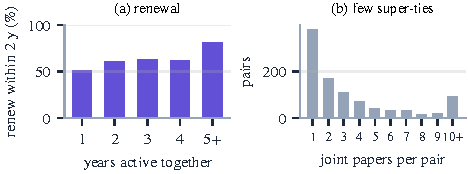
\includegraphics[width=\columnwidth]{figures/fig_ties.pdf}
\caption{(a) Share of faculty pairs that write together again within two years, by years already active together; (b) joint papers per pair.}
\label{fig:ties}
\end{figure}

\subsection{Spreading and synchronisation: theory vs simulation}
\textbf{SIR.} From~(\ref{eq:sir}), the mean-field estimate is $\beta_c^{MF}=\bmfT$ for Trichy ($\langle k\rangle=\kOneT$, $\langle k^2\rangle=\kTwoT$) and
\bmfS{} for Surathkal ($\langle k\rangle=\kOneS$, $\langle k^2\rangle=\kTwoS$); the spectral bound $1/\lambda_1$ is \bLamT{} and \bLamS{} ($\lambda_1=\lamOneT$, \lamOneS);
and the non-backtracking threshold is $\beta_c=\bcT$ and \bcS. The simulations take off close to the non-backtracking values (Fig.~\ref{fig:dyn}a,b): with random starters
the reach at $\beta=0.1/0.2/0.3$ is \reachT\% at Trichy and \reachS\% at Surathkal. Starting from hubs spreads further, and ideas spread more easily
at Surathkal, whose bigger connected hubs raise $\lambda$.

\textbf{Kuramoto.} Equation~(\ref{eq:kc}) gives $K_c=\KcT$ (Trichy) and \KcS{} (Surathkal), where $r$ starts to rise in the simulations
(Fig.~\ref{fig:dyn}c). Full synchrony is much harder than in random networks (Laplacian eigenratio \eigR{} vs \eigRw), because groups are joined by
thin bridges. The full derivations are in \texttt{dashboard/docs/threshold\_calculations.pdf}.

% ==============================================================================
\section{Main Findings and Comparison with Real Networks}
\label{sec:findings}
Table~\ref{tab:findings} lists \nPicked{} of our \nFindings{} findings (all are in \texttt{data/analysis/FINDINGS.md} and on the dashboard's Key
findings tab) with what they mean and how they compare with published real networks~\cite{newman2001, newman2002, barabasi2002, leskovec2005, libennowell2007}.


% ==============================================================================
\section{Limitations}
\label{sec:limits}
\begin{itemize}
\item OpenAlex coverage and affiliations are not perfect; about 95\% of automatic faculty matches were right in a hand-checked sample, and dropping
doubtful matches leaves the results unchanged.
\item Quartiles come from SCImago subject areas and IF is OpenAlex's 2-year mean citedness, not the JCR impact factor.
\item All comparisons are associations, not causes. The six-NIT results rest on six data points and on faculty lists with only today's staff.
\item The networks are small and faculty-only, while the published comparisons use networks of thousands of authors.
\end{itemize}

% ==============================================================================
\section{Conclusion}
\label{sec:conclusion}
The two NITs publish the same amount with the same field-weighted impact; Surathkal's higher output per person comes mostly from its more senior
faculty, and the real differences are by branch. Both co-authorship networks are small worlds organised by department, held together by a few
bridges, assortative like other social networks, and densify with shrinking distances like real growing networks ($a=\aExp$, within the range
of~\cite{leskovec2005}). New collaborations are predictable well above chance from a model trained on 2016--2022 alone, and spreading and
synchronisation start where network theory predicts.

{\footnotesize
\begin{thebibliography}{9}\setlength{\itemsep}{0pt}
\bibitem{leskovec2005} J.~Leskovec, J.~Kleinberg, C.~Faloutsos, ``Graphs over time: densification laws, shrinking diameters and possible explanations,'' \emph{Proc.\ KDD}, 177--187, 2005. doi:10.1145/1081870.1081893
\bibitem{newman2001} M.~E.~J. Newman, ``The structure of scientific collaboration networks,'' \emph{PNAS} 98(2), 404--409, 2001. doi:10.1073/pnas.98.2.404
\bibitem{barabasi2002} A.-L. Barab\'asi \emph{et al.}, ``Evolution of the social network of scientific collaborations,'' \emph{Physica A} 311, 590--614, 2002. doi:10.1016/S0378-4371(02)00736-7
\bibitem{newman2002} M.~E.~J. Newman, ``Assortative mixing in networks,'' \emph{Phys.\ Rev.\ Lett.} 89, 208701, 2002. doi:10.1103/PhysRevLett.89.208701
\bibitem{libennowell2007} D.~Liben-Nowell, J.~Kleinberg, ``The link-prediction problem for social networks,'' \emph{JASIST} 58(7), 1019--1031, 2007. doi:10.1002/asi.20591
\bibitem{karrer2014} B.~Karrer, M.~E.~J. Newman, L.~Zdeborov\'a, ``Percolation on sparse networks,'' \emph{Phys.\ Rev.\ Lett.} 113, 208702, 2014.
\bibitem{restrepo2005} J.~G. Restrepo, E.~Ott, B.~R. Hunt, ``Onset of synchronization in large networks of coupled oscillators,'' \emph{Phys.\ Rev.\ E} 71, 036151, 2005.
\end{thebibliography}}

\end{document}
